\section{Java enterprise edition}

Java Enterprise Edition (Java EE) serves as a platform designed for the creation, deployment, and maintenance of three-tier web applications.
\begin{figure}[H]
    \centering
    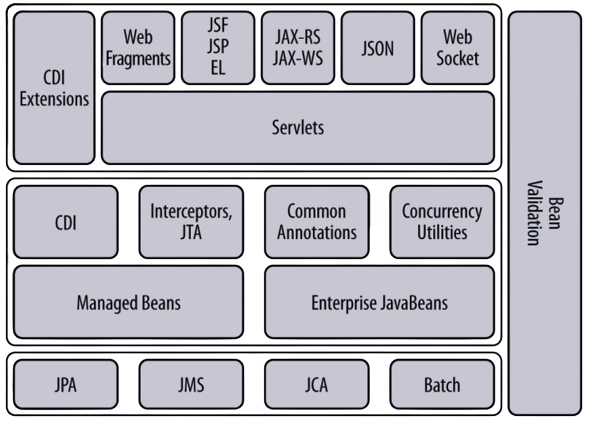
\includegraphics[width=0.75\linewidth]{images/jee.png}
\end{figure}

\paragraph*{Java Database Connectivity}
The JDBC API stands as the initial industry standard for establishing database-independent connectivity between Java and databases. 
Through JDBC, one can establish connections with databases, send SQL statements, and process the results.
    
\paragraph*{Servlets}
Servlets are  Java technologies employed in the presentation tier of web applications. 
 Servlets offer a platform-independent, component-based approach for constructing web-based applications. 
They have access to other Java APIs for interfacing with enterprise databases and operate within a container for concurrency control and lifecycle management.
    
\paragraph*{Jakarta Enterprise Beans}
EJB technology, utilized on the server side, enables the development of distributed, transactional, secure, and portable applications. 
EJB components facilitate interaction between the web front-end and business functions, as well as data access services.
    
\paragraph*{Java Persistence API}
JPA defines an interface for mapping relational data to objects in Java. 
It includes the API implementation package \texttt{javax.persistence}, the Java-compatible query language Java Persistence Query Language, and specifications for metadata defining object-relational mappings.
    
\paragraph*{Java Transaction API}
JTA manages transactions in Java, allowing components to initiate, commit, and rollback transactions in a resource-agnostic manner. 
With JTA, Java components can oversee multiple resources within a single transaction using a unified interaction model.

\begin{example}
    To extract data from a database using JPA we use: 
    \begin{lstlisting}[style=Java]
public List<Mission> findMissionsByUser(int userId) {
Reporter reporter = em.find(Reporter.class, userId);
List<Mission> missions = reporter.getMissions();
return missions;
}
    \end{lstlisting}
    To insert data in a database using JPA we use: 
    \begin{lstlisting}[style=Java]
public void createMission(Date startDate, int days, String destination, String description, int reporterId) {
Reporter reporter = em.find(Reporter.class, reporterId);
Mission mission = new Mission(startDate, days, destination, description, reporter);
reporter.addMission(mission);
em.persist(reporter);
}        
    \end{lstlisting}
    To modify data in a database using JPA we use: 
    \begin{lstlisting}[style=Java]
public void reportMission(int missionId, MissionStatus missionStatus) {
Mission mission = em.find(Mission.class, missionId);
mission.setStatus(MissionStatus.REPORTED);
}
    \end{lstlisting}
\end{example}